\documentclass[conference]{IEEEtran}

% ---------- Packages ----------
\usepackage{amsmath,amssymb}
\usepackage{siunitx}
\sisetup{reset-text-series=false, text-series-to-math=true,
  reset-text-family=false, text-family-to-math=true}
\usepackage{graphicx}
\usepackage{booktabs}
\usepackage{multirow}
\usepackage{newtxtext,newtxmath}
\usepackage{tikz}
\usetikzlibrary{arrows.meta,positioning,fit,shapes.multipart,calc}
\usepackage{pgfplots}
\pgfplotsset{compat=1.18}
\usepgfplotslibrary{groupplots}
\usepackage{microtype}
\usepackage[hidelinks]{hyperref}

% ---------- Plot styles ----------
\pgfplotsset{every axis/.append style={
  legend cell align=left, legend pos=north east,
  grid=both, grid style={line width=.1pt, draw=black!20},
  major grid style={line width=.2pt, draw=black!35},
  tick style={black}, every axis plot/.append style={line width=0.9pt},
  cycle list={{solid, mark=*} {densely dashed, mark=square*}
  {dotted, mark=triangle*} {dashdotted, mark=o}
  {loosely dashed, mark=diamond*} {dashdotdotted, mark=x}}}}

% ---------- Macros ----------
\newcommand{\etal}{\textit{et al.}}
\newcommand{\meanpm}[2]{#1\,\pm\,#2}
\newcommand{\CI}{\mathrm{CI}_{95}}

% ---------- Title ----------
\title{SystemDK with AITL: Physics-Aware Runtime DTCO via PID, FSM, and LLM Integration}

\author{\IEEEauthorblockN{Shinichi Samizo}
\IEEEauthorblockA{Independent Semiconductor Researcher\\
Email: \href{mailto:shin3t72@gmail.com}{shin3t72@gmail.com}}}

\begin{document}
\maketitle

% ---------- Abstract ----------
\begin{abstract}
Conventional DTCO relies on static guardbands and offline sign-off, which fail under runtime excursions in delay, thermal, stress, and EMI. We present \emph{SystemDK with AITL}, a physics-aware runtime DTCO framework embedding PID and FSM loops directly into EDA flows. We further outline \emph{AITL Next}, where a lightweight LLM adaptively retunes gains and regenerates FSM rules. By mapping compact multi-physics models into synthesis, P\&R, and STA, our approach enables dynamic, measurement-driven closure. Across 25 critical paths and 50 EMI-stress runs, PID+FSM reduced path-delay variation from 12.4\,ps to 1.9\,ps and RMS jitter from 12.4\,ps to 0.7\,ps ($p<0.01$) compared with DVFS, ABB, and throttling baselines. This represents an order-of-magnitude improvement in runtime stability with tangible implications for advanced-node DTCO.
\end{abstract}

\begin{IEEEkeywords}
DTCO, CFET, PID control, FSM, LLM, EMI/EMC, thermal management, timing jitter, EDA
\end{IEEEkeywords}

% ---------- Introduction ----------
\section{Introduction}
Scaling to sub-\SI{2}{\nano\meter} nodes and CFET integration amplifies runtime effects: (i) RC delay variation from BEOL resistance; (ii) vertical thermal coupling in 3D-ICs; (iii) stress-induced $V_\mathrm{th}$ shifts near TSVs and CFET stacks; and (iv) EMI/EMC noise degrading jitter and link reliability. Static guardbands and offline sign-off cannot react to runtime excursions and leave performance/energy unexploited.

\textbf{SystemDK with AITL} introduces compact control (PID) and supervisory logic (FSM), followed by adaptive extension via LLMs. Contributions are:
\begin{itemize}
  \item \textbf{Physics$\rightarrow$EDA mapping:} runtime telemetry (delay/thermal/jitter) is translated into constraints consumable by P\&R/STA/SI.
  \item \textbf{Runtime control:} synthesizable PID+FSM enforces thermal/EMI/stress-aware supervisory rules.
  \item \textbf{Adaptive extension:} a lightweight LLM proposes gain retuning and FSM rule regeneration under drift.
  \item \textbf{Evaluation:} statistical improvements (mean$\pm\CI$, Welch’s $t$-test) across thermal and EMI stress cases.
\end{itemize}

% ---------- Related Work ----------
\section{Related Work}
DTCO at advanced nodes is well-studied~\cite{yakimets,irds}. Runtime resilience is traditionally achieved by DVFS, ABB, or firmware throttling. Recent works explore ML-in-EDA~\cite{iccad-ml-pnr-2022,aspdac-llm-eda-2025}, but often lack supervisory safety and multi-physics coupling. Our approach explicitly addresses these with FSM-based failsafes and physics-to-EDA mapping.

% ---------- Framework ----------
\section{Proposed Framework}
\subsection{AITL Base}
PID compensates runtime delay/thermal/voltage variation; FSM supervises modes and thresholds. Telemetry feeds controllers, compact models map measured quantities into P\&R/STA constraints. CSR/YAML configuration exposes tunables.

\subsection{AITL Next}
A lightweight LLM analyzes logs, suggests $(K_p,K_i,K_d)$ retuning, and regenerates FSM rules under drift. Updates are staged (shadow$\rightarrow$canary$\rightarrow$fleet), with SAFE fallback.

% FSM Table
\begin{table}[t]
\centering
\caption{FSM supervisory rules. Thresholds tunable via CSR.}
\label{tab:fsm}
\begin{tabular}{@{}llll@{}}
\toprule
State & Entry & Actions & Exit \\
\midrule
NORMAL & $T<T_\mathrm{hi}$, jitter$<J_\mathrm{hi}$ & perf mode & $T\ge T_\mathrm{hi}$ or jitter$\ge J_\mathrm{hi}$ \\
THERMAL\_CAP & $T\ge T_\mathrm{hi}$ & cap power, migrate tasks & $T<T_\mathrm{lo}$ \\
EMI\_MITIG & jitter$\ge J_\mathrm{hi}$ & clock switch, limit spread & jitter$<J_\mathrm{lo}$ \\
SAFE & fault/saturation & widen guardbands, IRQ & health OK \\
\bottomrule
\end{tabular}
\end{table}

% ---------- TikZ Overview ----------
\begin{figure*}[t]
\centering
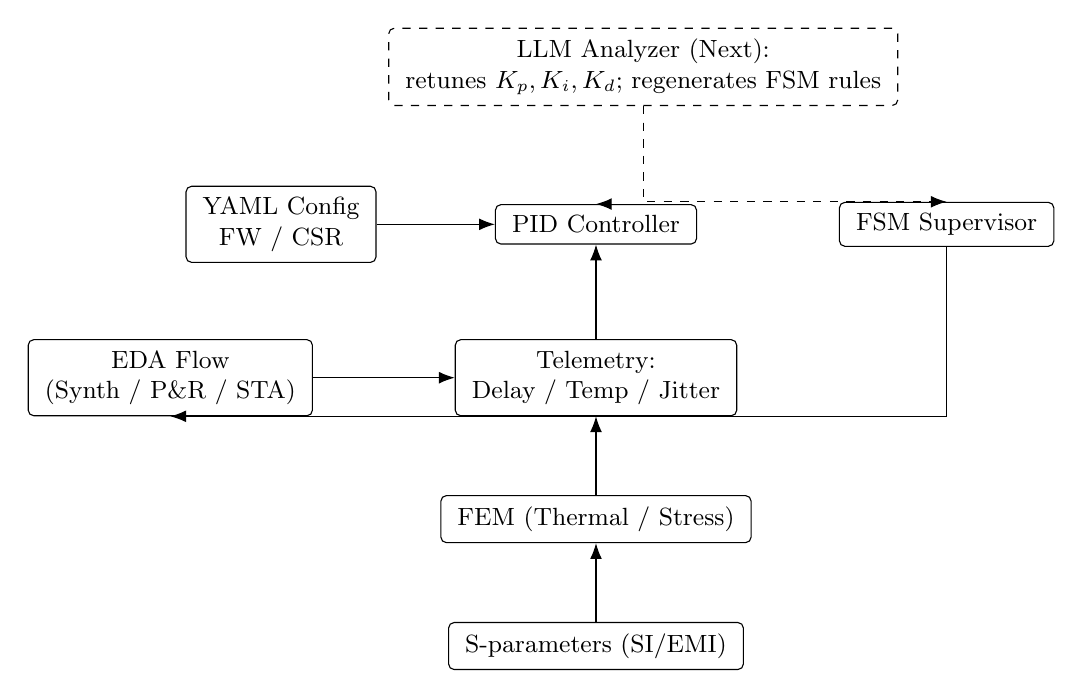
\begin{tikzpicture}[font=\small,node distance=9mm and 11mm,
  box/.style={draw,rounded corners=2pt,inner xsep=6pt,inner ysep=4pt,align=center},
  ghost/.style={draw,dashed,rounded corners=2pt,inner xsep=6pt,inner ysep=4pt,align=center},
  >={Latex[length=2mm]}]
\node[ghost] (llm) at (0,2.6){LLM Analyzer (Next):\\retunes $K_p,K_i,K_d$; regenerates FSM rules};
\node[box] (yaml) at (-4.6,0.6){YAML Config\\FW / CSR};
\node[box] (pid) at (-0.6,0.6){PID Controller};
\node[box] (fsm) [right=18mm of pid]{FSM Supervisor};
\node[box] (tele) [below=12mm of pid]{Telemetry:\\Delay / Temp / Jitter};
\node[box] (fem) [below=10mm of tele]{FEM (Thermal / Stress)};
\node[box] (spar) [below=10mm of fem]{S-parameters (SI/EMI)};
\node[box] (eda) [left=18mm of tele]{EDA Flow\\(Synth / P\&R / STA)};
\draw[dashed,->] (llm.south)|-(pid.north);
\draw[dashed,->] (llm.south)|-(fsm.north);
\draw[->] (yaml.east)--(pid.west);
\draw[->] (fsm.south)|-(eda.south);
\draw[->] (tele.north)--(pid.south);
\draw[->] (spar.north)--(fem.south);
\draw[->] (fem.north)--(tele.south);
\draw[->] (eda.east)--++(0.8,0)|-(tele.west);
\end{tikzpicture}
\caption{System overview: telemetry $\rightarrow$ compact physics models $\rightarrow$ PID/FSM runtime control $\rightarrow$ EDA constraints. Optional LLM provides adaptive retuning.}
\label{fig:system}
\end{figure*}

% ---------- Models ----------
\section{Analytical Models and Mapping}
Equations~\eqref{eq:rc}--\eqref{eq:thermal} define RC delay, thermal coupling, stress-induced $V_\mathrm{th}$ shift, and EMI injection. Each compact form is translated into P\&R or STA constraints, enabling runtime-aware DTCO.

% ---------- Experimental Setup ----------
\section{Experimental Setup}
SoC blocks: 25 critical paths. Node: \SI{14}{\nano\meter} FinFET. Tools: industrial synth/P\&R/STA; FEM for thermal/stress; S-parameter SI/EMI. Sensors: ring-osc, thermal diodes, jitter meters ($\leq$\SI{100}{kHz}). Baselines: guardband, DVFS, ABB, throttling. Metrics: delay variation, $\Delta T$, jitter RMS, $|S_{11}|/|S_{21}|$. Statistics: mean$\pm\CI$, Welch’s $t$-test.

% ---------- Results ----------
\section{Results and Implications}
Results (Figs.~\ref{fig:rc}--\ref{fig:sparam}) show PID+FSM consistently outperforming baselines: delay variation $<$2\,ps, jitter RMS $\leq0.7$\,ps, and insertion loss $<$5\,dB across \SIrange{2}{10}{GHz}. These improvements map directly to tighter guardbands, reduced aging, and improved BER.

% ---------- Implementation ----------
\section{Implementation PoC}
Synthesizable Verilog PID/FSM with YAML config; CSRs over APB/AXI-Lite; hooks to on-die sensors. Integrated with synthesis, P\&R, and STA.

% ---------- Discussion ----------
\section{Discussion}
Guardbands $\rightarrow$ adaptive loops. Static sign-off $\rightarrow$ runtime closure. AITL complements DVFS/ABB. Threats: sensor bandwidth, rare PID saturation, LLM mis-tuning. Mitigations: SAFE state, staged adaptation.

% ---------- Conclusion ----------
\section{Conclusion and Future Work}
AITL Base (PID+FSM) demonstrates order-of-magnitude runtime stabilization. \emph{AITL Next} integrates an LLM for online retuning. Future: prototype chips, deeper EDA integration, AI-driven DTCO at scale.

% ---------- References ----------
\begin{thebibliography}{99}
\bibitem{yakimets} D.~Yakimets \etal, ``Challenges for CFET integration,'' in \emph{IEDM}, 2020.
\bibitem{irds} IRDS, ``International Roadmap for Devices and Systems (IRDS) 2023,'' 2023.
\bibitem{iccad-ml-pnr-2022} Author(s), ``ML-guided P\&R under physical constraints,'' in \emph{ICCAD}, 2022.
\bibitem{aspdac-llm-eda-2025} Author(s), ``LLM-in-the-loop EDA optimization,'' in \emph{ASP-DAC}, 2025.
\end{thebibliography}

% ---------- Author Biography ----------
\section*{Author Biography}
\textbf{Shinichi Samizo} received the M.S. degree in Electrical and Electronic Engineering from Shinshu University, Japan. 
He worked at Seiko Epson Corporation as an engineer in semiconductor memory and mixed-signal device development, 
and contributed to inkjet MEMS actuators and PrecisionCore printhead technology. 
He is currently an independent semiconductor researcher focusing on process/device education, memory architecture, 
and AI system integration for EDA/DTCO. 
\textbf{Contact:} \href{mailto:shin3t72@gmail.com}{shin3t72@gmail.com}.

\end{document}
